\documentclass[sigconf,anonymous,review]{acmart}
% B full controls: figure-size proof only; no scientific manuscript body.
\setcopyright{none}
\settopmatter{printacmref=false}
\acmConference[WWW '27]{The ACM Web Conference 2027}{May 10--14, 2027}{Dublin, Ireland}
\acmYear{2027}
\copyrightyear{2027}
\acmDOI{}
\acmISBN{}
\usepackage{graphicx}
\usepackage{microtype}
\title{B full controls: figure-size proof only}
\author{Anonymous Authors}
\begin{document}
\pagestyle{plain}
\twocolumn
\typeout{PROOF-TEXTWIDTH-PT=\the\textwidth}
\typeout{PROOF-COLUMNWIDTH-PT=\the\columnwidth}
\typeout{PROOF-TEXTHEIGHT-PT=\the\textheight}
\begin{figure*}[p]
\centering
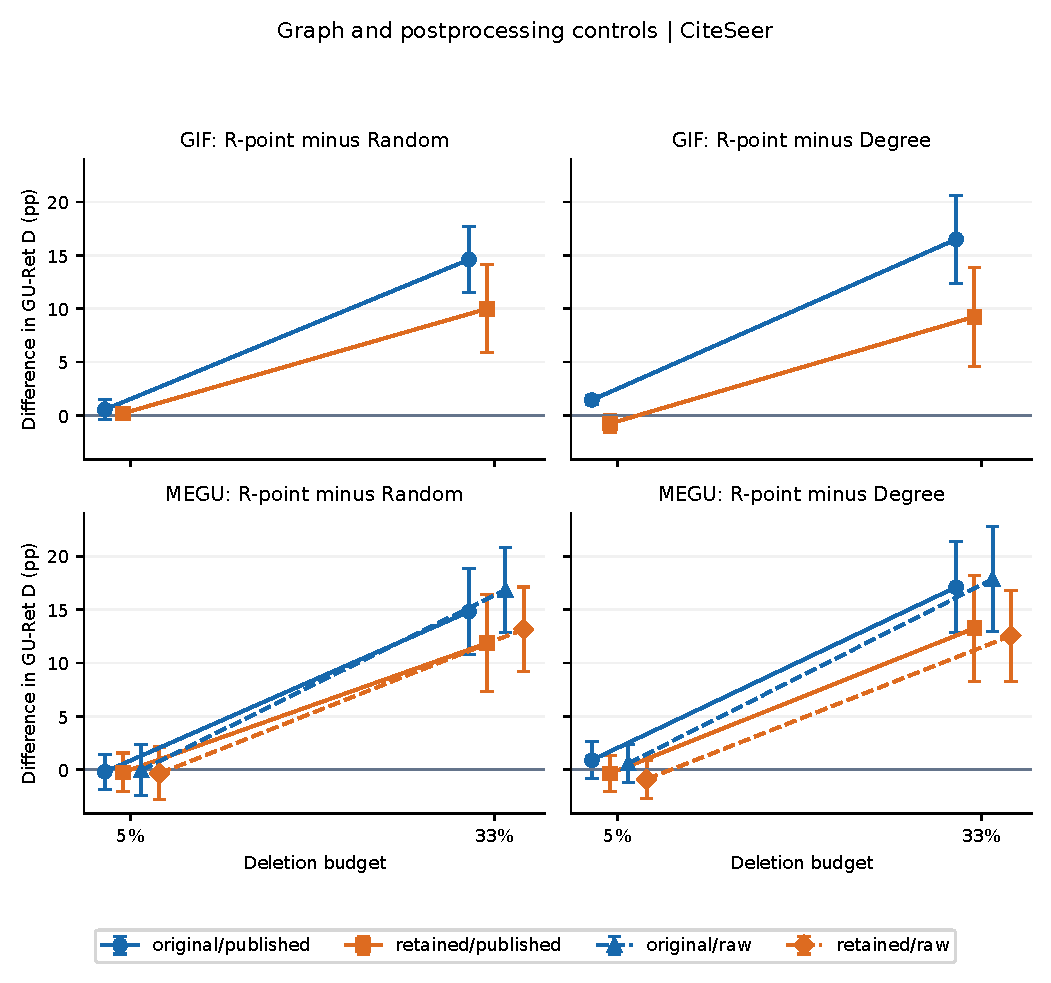
\includegraphics[width=\textwidth]{images/strategy_graph_controls.pdf}
\caption{Size proof only: request differences on two evaluation graphs.
CiteSeer/GCN, fixed split, GIF and MEGU, three joint seeds, 5\% and 33\% node deletion.
Points are R-point minus Random or Degree GU--Retrain disagreement differences in percentage points; error bars are sample standard deviations.
The 33\% direction persists, while magnitudes depend on the graph and GIF's 5\% comparison with Degree reverses sign.
Two selected budgets do not establish seven-budget monotonicity.
GIF raw equals published and is displayed once; MEGU matched C\&S changes only Original, so its unchanged GU--Retrain distance is definitional and is not an additional robustness check.
Shared requests and Retrain endpoints do not create independent repetitions.}
\Description{Four panels display two-baseline request differences at both budgets, with original and retained graphs and MEGU raw or published postprocessing.}
\end{figure*}
\clearpage
\begin{figure*}[p]
\centering
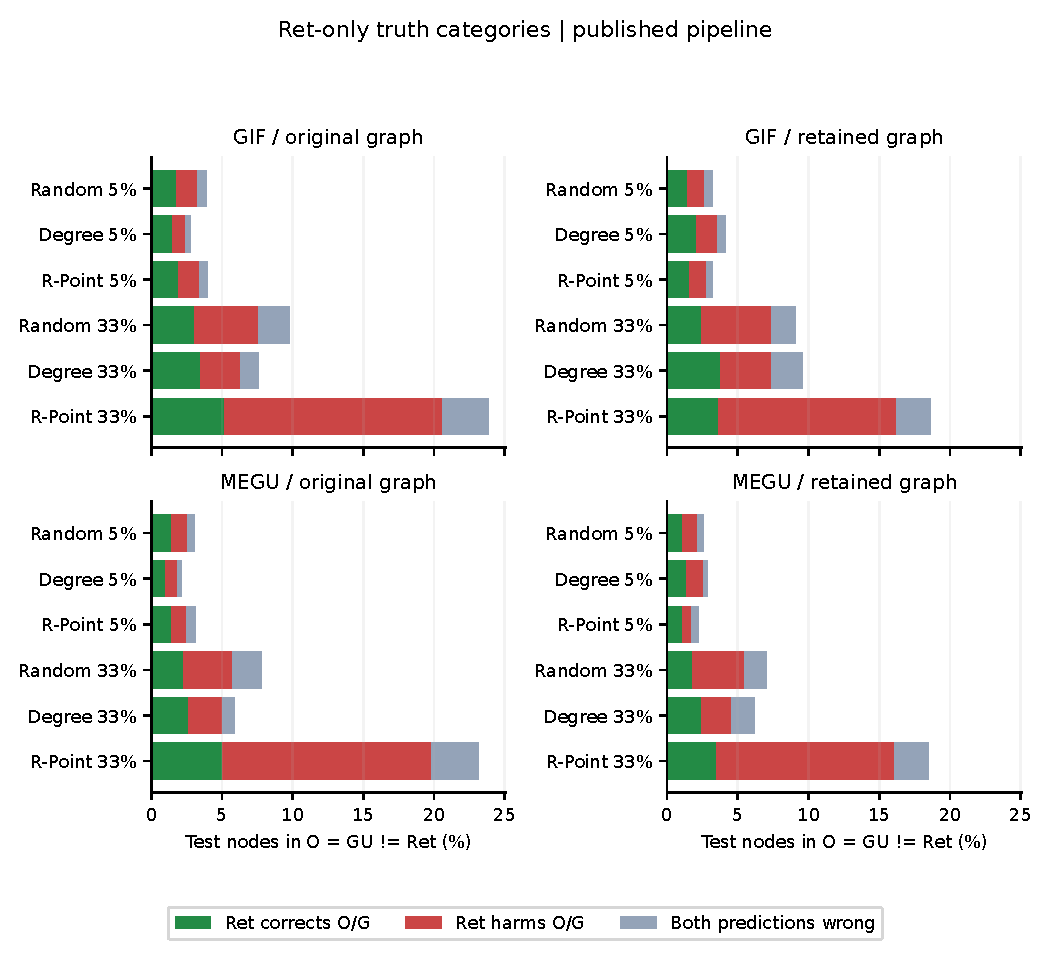
\includegraphics[width=\textwidth]{images/ret_only_truth.pdf}
\caption{Size proof only: truth-aware Ret-only categories for all three strategies, both budgets, and both graphs.
Each segment is a mean count divided by the same 666 test nodes, averaged equally over three seeds.
The total bar covers only Ret-only nodes and is not total GU--Retrain disagreement.
Ret-only denotes $O=G\ne R$ and includes Retrain corrections, losses, and both-wrong predictions; this is a descriptive partition, not causal attribution or a forgetting certificate.
The large-budget R-point relation does not extend to 5\% MEGU.
MEGU uses the published pipeline in this plot; its raw Original and updated+C\&S GU endpoints must be distinguished from the matched-Original control.}
\Description{Four panels retain both methods and both graphs, showing Ret-only truth categories for all strategies and budgets.}
\end{figure*}
\clearpage
\begin{figure*}[p]
\centering
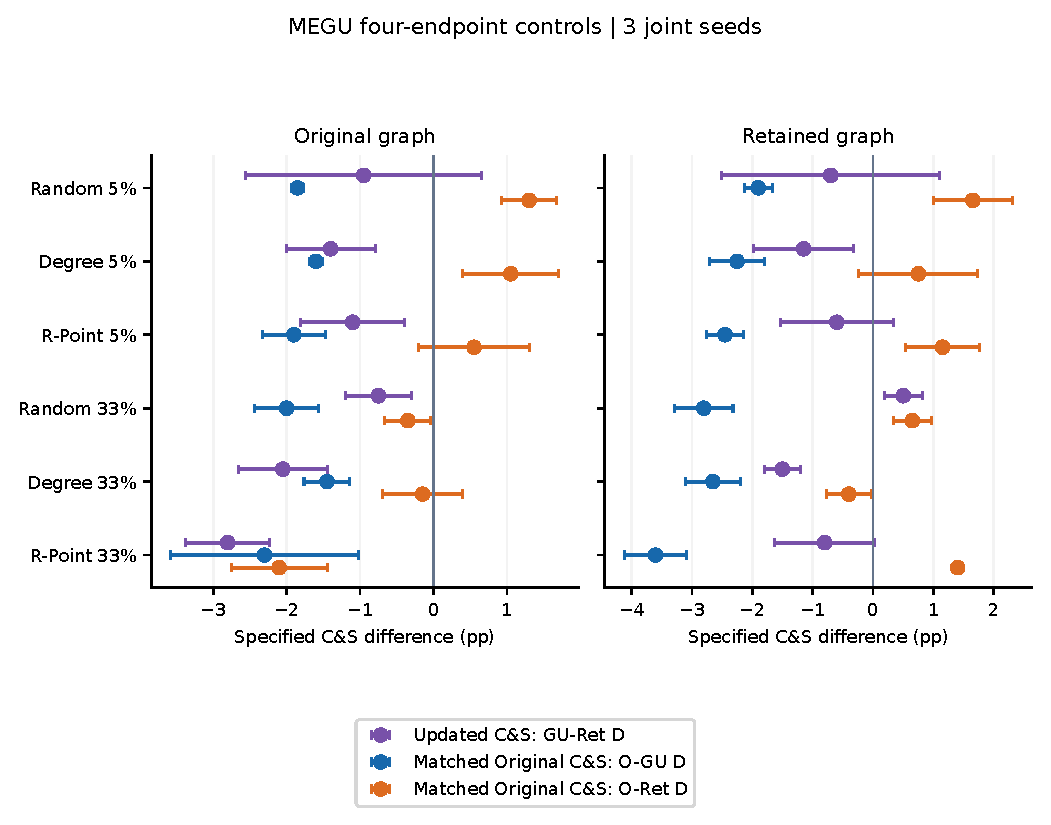
\includegraphics[width=\textwidth]{images/megu_cs_controls.pdf}
\caption{Size proof only: MEGU postprocessing changes and matched-Original relations.
All three strategies, two budgets, and both graphs are retained; points are three-seed means and bars are sample standard deviations.
Raw-to-C\&S changes can be nonzero, including a $+0.501$ pp GU--Retrain difference change for Random at 33\% on the retained graph.
Matched C\&S changes Original to Original+C\&S while holding GU and Retrain fixed; identical GU--Retrain distance is therefore definitional.
The two panel axes may use different ranges; compare percentage-point ticks, not pixel lengths.
These graph and postprocessing controls do not establish Retrain training quality, causal mechanisms, population generality, or the paper's writing gate.}
\Description{MEGU panels compare no-update and updated C-and-S effects and changes in Original-related disagreements across both evaluation graphs.}
\end{figure*}
\clearpage
\end{document}
